\chapter{Qualitative Methods, Numerical Methods, and Bifurcations}
\section{Equilibrium Points and Stability}
A first order autonomous differential equation may have an equilibrium point where the
change simply stops.  In this section we will build (or remind you about) the tools to
find and analyze equilibrium points for autonomous first order differential equations.

\begin{problem}
    The equilibrium point of a first order autonomous differential equation $y'(t) = f(y)$ is defined as
    the value of $y$ where $y'=0$.  
    \begin{itemize}
        \item[(a)] Why is this called an equilibrium point?
        \item[(b)] Find the equilibrium for the first order autonomous differential equation
            \[ y' = -0.2y^2 + 3 \]
        \item[(c)] Make a plot with $y'$ on the vertical axis on $y$ on the horizontal axis for
            the previous differential equation.  Use this plot to determine whether the
            equilibrium point is stable or unstable.
    \end{itemize}
\end{problem}
\solution{
    The equilibrium is $y_{eq} = \sqrt{3/0.2} = \sqrt{15}$.  Stable
}


\begin{problem}
    The air resistance on a sky diver is proportional to the \underline{square} of the velocity.
    Newton's 2nd law can be used to get a differential equation for the velocity of the
    sky diver.
    \begin{enumerate}
        \item Write the differential equation for the velocity (take {\it down} to be
        positive).  You might want to start with a free body diagram and consider the
        balance of forces.  \ldots What Would Newton Do? (WWND)
        \item Find the equilibrium (AKA: terminal velocity) in terms of the mass and the
            proportionality constant for air resistance. How many equilibria are there?
            Discuss their stability.
    \end{enumerate}
\end{problem}
\solution{
    \[ mv' = mg - kv^2 \]
    \[v_{eq} = \sqrt{\frac{mg}{k}} \]
    So for every $k$ there is a terminal velocity, but as $k$ gets larger the terminal
    velocity goes down.
}


\begin{problem}
    Create a first order autonomous differential equation that has 2 unstable equilibria
    and 1 stable equilibrium.\\
    Hint\#1: Use the plot of $y'$ vs $y$ to help.\\
    Hint\#2: Write the right-hand side of your DE to in factored form.
\end{problem}
\solution{
$y' = (y-1)(y-2)(y-3)$ will be unstable at $y=1$ and $y=3$ but stable at $y=2$.
}


\begin{problem}
    A trout pond has a carrying capacity of 200 fish.  Suppose that the trout population
    can be modeled according to the logistic equation
    \[ \frac{dP}{dt} = kP\left( 1-\frac{P}{200} \right) \]
    where $k$ is the intrinsic growth rate of the population.  For the sake of simplicity
    in this model let's assume that $k = 0.5$ (for now).  
    \begin{enumerate}
        \item[(a)] The coordinate axes below have $dP/dt$ on the vertical axis and $P$ on
            the horizontal axis.  Use the differential equation to sketch this plot.
            \begin{center}
                \begin{tikzpicture}
                    \draw[->,thick, black] (0,0) -- (5,0) node[anchor=west]{$P$};
                    \draw[->,thick, black] (0,-1) -- (0,3)
                    node[anchor=south]{$\frac{dP}{dt}$};
                \end{tikzpicture}
            \end{center}
        \item[(b)] Mark the intercepts on the horizontal axis in the plot above.  What do
            they represent in the context of this problem?
        \item[(c)] What does it mean about the rate of change of the population if  the
            plot lies above the horizontal axis?  What about below?
        \item[(d)] Use your answer in part (c) to classify the two equilibrium points as
            either stable or unstable.
    \end{enumerate}
\end{problem}
\solution{
    \begin{enumerate}
        \item[(a)] This is a downward facing parabola with roots at 0 and 200.
        \item[(b)] The intercepts are where $P'=0$ so the rate of change is zero.  These
            are the equilibrium points.
        \item[(c)] If the curve is above the horizontal axis then the rate of change is
            positive.  If the curve is below the horizontal axis then the rate of change
            is negative.
        \item[(d)] 0 is unstable and 200 is stable.
    \end{enumerate}
}


\begin{problem}
    Use what you learned in the previous problems to find and classify the equilibria for the
    first order non-linear autonomous differential equation
    \[ y'(t) = (y-1)(y-2)(y-3)^2. \]
\end{problem}
\solution{
1 is stable, 2 is unstable and 3 is semi-stable
}

\begin{technique}[Phase Line Analysis]
    It is often very helpful to draw a {\it phase diagram} (sometimes called a phase line)
    to analyze the equilibrium points of an autonomous differential equation.  There are
    four possible cases shown graphically in Figure \ref{fig:phaseline}.  In each of the
    following fill in with the word(s) ``stable'', ``unstable'', ``semi-stable approaching
    from below'', or ``semi-stable approaching from above''.
    \begin{itemize}
        \item In Case \#1 there is a/an \underline{\hspace{1.5in}} equilibrium at $y=2$.
        \item In Case \#2 there is a/an \underline{\hspace{1.5in}} equilibrium at $y=2$.
        \item In Case \#3 there is a/an \underline{\hspace{1.5in}} equilibrium at $y=2$.
        \item In Case \#4 there is a/an \underline{\hspace{1.5in}} equilibrium at $y=2$.
    \end{itemize}
\end{technique}
\solution{
    \begin{itemize}
        \item Case \#1: unstable
        \item Case \#2: semi-stable approaching from below
        \item Case \#3: stable 
        \item Case \#2: semi-stable approaching from above
    \end{itemize}
}

\begin{figure}
    \begin{center}
        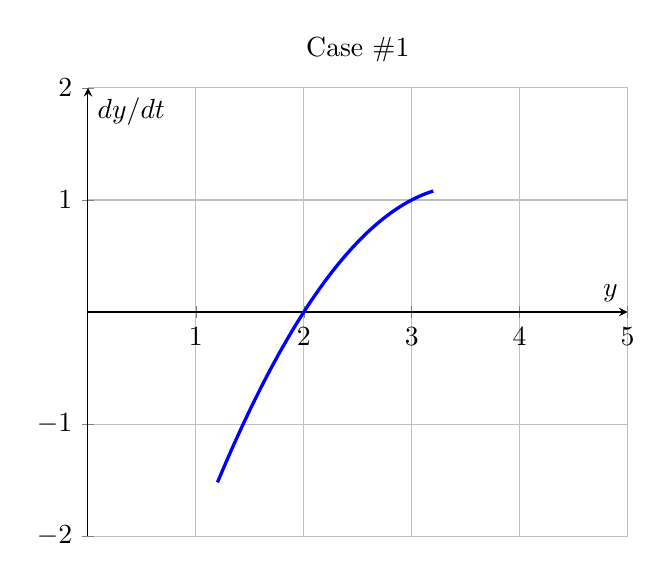
\begin{tikzpicture}
            \begin{axis}[axis lines=center, grid, domain=0:5, xlabel={$y$},
                    ylabel={$dy/dt$}, title={Case \#1}, xmin=0, xmax=5, ymin=-2, ymax=2]
                    \addplot[blue, domain=1.2:3.2, very thick, smooth] {-0.5*(x-2)*(x-5)};
            \end{axis}
        \end{tikzpicture}
        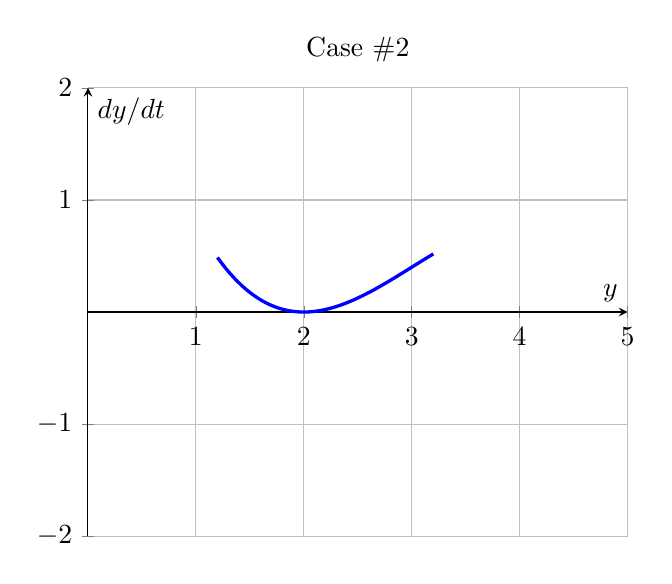
\begin{tikzpicture}
            \begin{axis}[axis lines=center, grid, domain=0:5, xlabel={$y$},
                    ylabel={$dy/dt$}, title={Case \#2}, xmin=0, xmax=5, ymin=-2, ymax=2]
                    \addplot[blue, domain=1.2:3.2, very thick, smooth] {-0.2*(x-2)^2*(x-5)};
            \end{axis}
        \end{tikzpicture}
        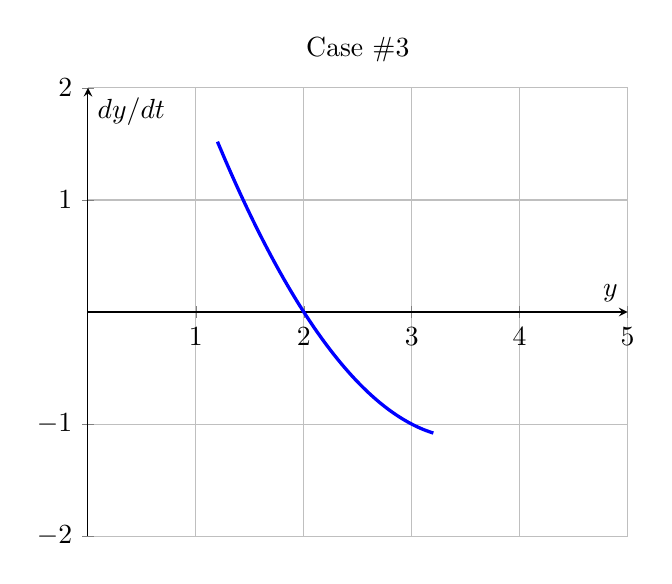
\begin{tikzpicture}
            \begin{axis}[axis lines=center, grid, domain=0:5, xlabel={$y$},
                    ylabel={$dy/dt$}, title={Case \#3}, xmin=0, xmax=5, ymin=-2, ymax=2]
                    \addplot[blue, domain=1.2:3.2, very thick, smooth] {0.5*(x-2)*(x-5)};
            \end{axis}
        \end{tikzpicture}
        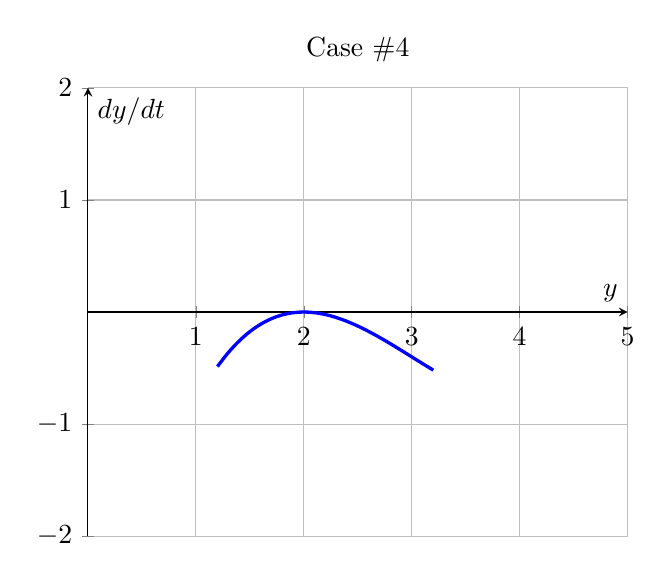
\begin{tikzpicture}
            \begin{axis}[axis lines=center, grid, domain=0:5, xlabel={$y$},
                    ylabel={$dy/dt$}, title={Case \#4}, xmin=0, xmax=5, ymin=-2, ymax=2]
                    \addplot[blue, domain=1.2:3.2, very thick, smooth] {0.2*(x-2)^2*(x-5)};
            \end{axis}
        \end{tikzpicture}
    \end{center}
    \caption{Four cases for phase line analysis. In each plot we see a small portion of
        the $\frac{dy}{dt}$ vs $y$ plot for an autonomous first order differential
        equation: $\frac{dy}{dt} = f(y)$.}
    \label{fig:phaseline}
\end{figure}


\begin{problem}
    For each of the phase plots in Figure \ref{fig:phase2} sketch a plot on the  $y$ vs
    $t$ plane of the solutions
    to the underlying differential equation. A few helpful markers are given to
    you in the first plot.
\end{problem}

\begin{figure}
    \begin{center}
        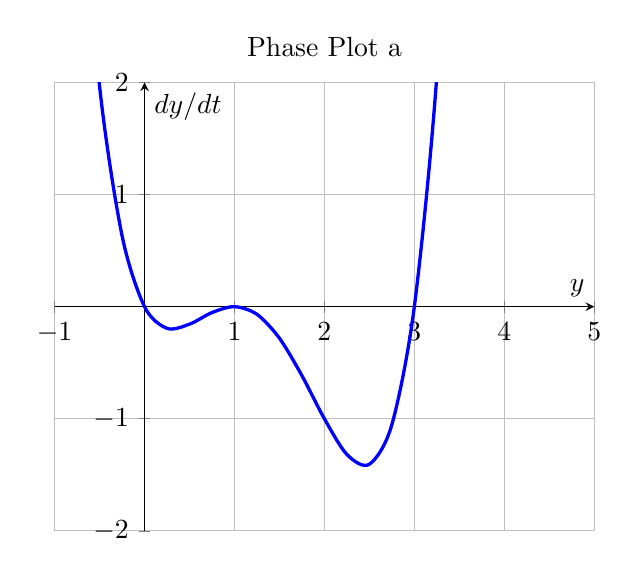
\begin{tikzpicture}
            \begin{axis}[axis lines=center, xlabel={$y$}, ylabel={$dy/dt$}, grid, xmin=-1,
                xmax=5, ymin=-2, ymax=2, title={Phase Plot a}]
                \addplot[smooth, very thick, blue, domain=-1:5] {0.5*x*(x-1)^2*(x-3)};
            \end{axis}
        \end{tikzpicture}
        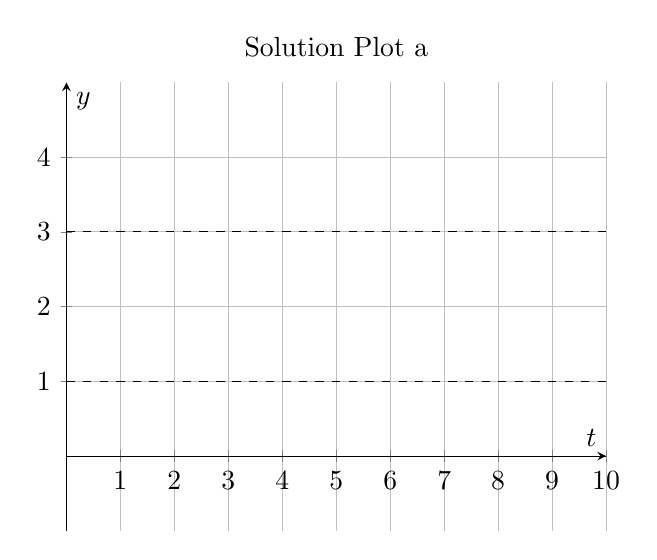
\begin{tikzpicture}
            \begin{axis}[axis lines=center, xlabel={$t$}, ylabel={$y$}, grid, xmin=0,
                xmax=10, ymin=-1, ymax=5, title={Solution Plot a}, ytick={1,2,3,4},
            xtick={1,2,3,4,5,6,7,8,9,10}]
                \addplot[dashed, domain=0:10] {0*x+0};
                \addplot[dashed, domain=0:10] {0*x+1};
                \addplot[dashed, domain=0:10] {0*x+3};
            \end{axis}
        \end{tikzpicture}
        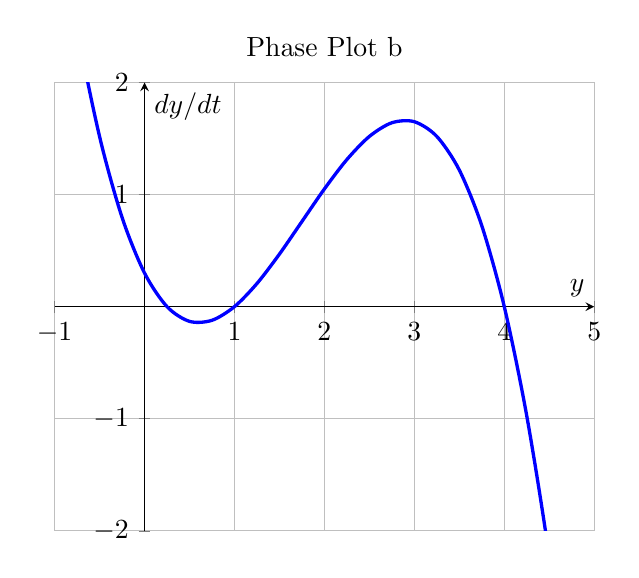
\begin{tikzpicture}
            \begin{axis}[axis lines=center, xlabel={$y$}, ylabel={$dy/dt$}, grid, xmin=-1,
                xmax=5, ymin=-2, ymax=2, title={Phase Plot b}]
                \addplot[smooth, very thick, blue, domain=-1:5] {-0.3*(x-0.25)*(x-1)*(x-4)};
            \end{axis}
        \end{tikzpicture}
        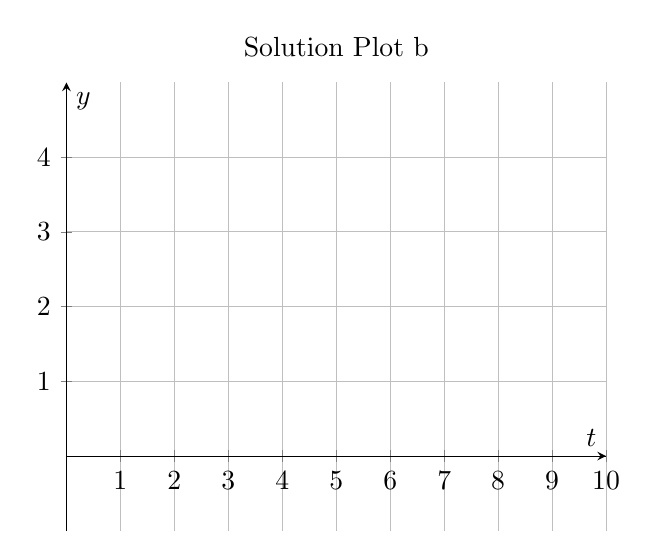
\begin{tikzpicture}
            \begin{axis}[axis lines=center, xlabel={$t$}, ylabel={$y$}, grid, xmin=0,
                xmax=10, ymin=-1, ymax=5, title={Solution Plot b}, ytick={1,2,3,4},
            xtick={1,2,3,4,5,6,7,8,9,10}]
                \addplot[smooth, domain=0:10] {0*x+0};
            \end{axis}
        \end{tikzpicture}
    \end{center}
    \caption{Phase plots and solution plots.  On the left are the phase plots and on the
    right are coordinate axes to sketch the solution plots.}
    \label{fig:phase2}
\end{figure}

\newpage


\newpage\section{Numerical Methods}

In this section we will build two numerical solvers that allow you to use a computer to
approximate solutions to the differential equation 
\begin{flalign}
    y' = f(t,y) \label{eqn:ode}
\end{flalign}
for a given initial condition.  In the problems that follow you will be creating several
\texttt{MATLAB} files that you will use throughout the course, so please save them in a
meaningful place and share them with your group mates.

\subsection{Euler's Method}
Euler's method is the simplest numerical method for solving the differential equation
$y'=f(t,y)$, and hence it is the best place to start!  You should be familiar with Euler's
method from pre-requisite courses, but this time we are not going to be using Excel (since
we usually need something FAR more powerful!).  

Euler's method is simple: approximate the derivative in the most naive possible way:
\[ \frac{dy}{dt} \approx \frac{y_{new} - y_{old}}{\Delta t} \]
and then rewrite the differential equation \eqref{eqn:ode} as
\[ \frac{y_{new} - y_{old}}{\Delta t} \approx f(t_{old},y_{old}). \]
After some rearrangement and relabeling we get the difference equation
\[ y_{n+1} = y_n + \Delta t f(t_n,y_n). \]

\begin{technique}[Euler's Method]
    To approximate $y' = f(t,y)$ first choose $\Delta t$ and then implmenet the difference
    equation
    \[ y_{n+1} + y_n + \Delta t f(t_n,y_n) \]
    using appropriate computer software. 
\end{technique}
Remember that the only reasonble choice for
$\Delta t$ is to make it {\it very small}.  The trade off to choosing $\Delta t$ small
is that it will take more computer memory to approximate the problem.


\begin{problem}
    In Excel the process of building an Euler solver is relatively simple.  In \texttt{MATLAB}
it takes a bit more work the very first time, but trust me, the work will pay off in the
long run!
\begin{enumerate}
    \item[(a)] Open \texttt{MATLAB} and create a new \underline{function}.  
    \item[(b)] Change the first line of the function so that it reads \\
        \texttt{function [t,y] = MyEuler(f,tmin,tmax,numpoints,IC)}
    \item[(c)] After the commented lines (which we'll come back to) you should complete the following
        code.  Explain what each line of code does using comments. Some of the lines of
        code are likely new to you so I suggest you either use the help command or you do
        some basic experimentation.
\begin{verbatim}
function [t,y] = MyEuler(f,tmin,tmax,numpoints,IC)
t=linspace(tmin,tmax,numpoints);  % what does this line do?
dt=t(2)-t(1); % what does this line do?
y=zeros(size(t)); % what does this line do?
y(1) = IC; % what does this line do?
for n=1:length(t)-1 % what does this line do?
    y(n+1) = ... some code for Euler's method ...
end
\end{verbatim}
    \item[(d)] Now.  Save this code in the working directory for this lab.  You also need to
        get \texttt{MATLAB} to look in that working directory.  The simplest way to do
        that is to press F5 while you're in the MyEuler function (and then ignore all of
        the errors that occur).  

        The code you just created works for ALL of the times that you ever need Euler's
        method.  We now just need to create a short script which calls this code and uses
        it.
    \item[(e)] Finally, let's try out your MyEuler code (and at this point you should see why
        you really shouldn't be using Excel for numerical differential equation solvers).
        I'm assuming that you have \texttt{MATLAB} working in the correct directory
        (you'll get errors otherwise!!).  

        We want to get an approximate solution to the differential equation
        \[ y' = -y \cdot \left( 1-\frac{y}{5} \right) + 0.1 t \quad \text{where} \quad
            y(0)=2 \]
            Open a new \underline{script} in \texttt{MATLAB} and complete the following code to get your
        plot.
\begin{verbatim}
clear; clc; clf;
f = @(t,y) -y*(1-y/5)+0.1*t;
[t,y] = MyEuler(f, ..., ..., ..., ...)
plot(t,y)
\end{verbatim}
    \item[(f)] Run your code for several different initial conditions and overlay the plots to
        explore the dynamics of the differential equation. Be sure to properly label your
        plot. It is probably best to do this step within a loop in MATLAB.  To get a
        legend to appear for each new plot you can use the following:
\begin{verbatim}
clear; clc; clf;
f = @(t,y) -y*(1-y/5)+0.1*t;
LegendItems = { }; % initialize the storage for the legend entries
counter=1; % set up a dummy counter
for IC= ... : ... : ...
  [t,y] = MyEuler(f, ..., ..., ..., ...)
  plot(t,y), hold on
  LegendItems{counter} = ['IC = ' , num2str(IC)]; % what does this line do?
  counter = counter+1; % what does this line do?
end
legend(LegendItems)
\end{verbatim}
\end{enumerate}
\end{problem}

\begin{problem}
    Run an Euler solver on the differential equation
        \[ y' = -y\left( 1-\frac{y}{5} \right)^2 + \sin(t) \]
        for several different initial conditions. Save your plot in an appropriate place
        with appropriate labels and title.
\end{problem}

\subsection{Runge-Kutta Method}
Euler's method is one of MANY different numerical differential equation solvers.  The
second one that we are going to study in this section is called the Runge-Kutta 4 solver.
The idea is basically the same as with Euler's method: approximate the derivative and
rewrite the differential equation as a difference equation.  The
difference here is that the algorithm is a bit more complex.  \dots Here it is:\\

\begin{technique}[Runge Kutta Method]
First define the dummy variables $k_1, k_2, k_3,$ and $k_4$ as
\begin{flalign*}
    k_1 &= f(t_n,y_n) \\
    k_2 &= f(t_n+\frac{\Delta t}{2} , y_n + \frac{\Delta t}{2} k_1) \\
    k_3 &= f(t_n+\frac{\Delta t}{2} , y_n + \frac{\Delta t}{2} k_2) \\
    k_4 &= f(t_n+\Delta t , y_n + \Delta t k_3).
\end{flalign*}
Then we build the difference equation as a weighted sum of the $k_j's$:
\begin{flalign*}
    y_{n+1} &= y_n + \frac{\Delta t}{6} \left( k_1 + 2 k_2 + 2k_3 + k_4 \right).
\end{flalign*}
% See Figure \ref{fig:RK_figure} to show the technique graphically.
\end{technique}

\begin{problem}
    Explain the Runge Kutta method graphically.
\end{problem}

% \begin{figure}[ht!]
%     \begin{center}
%         \begin{tikzpicture}
%             \begin{axis}[axis lines=center, xmin=0, xmax=3.5, ymin=0,
%                     ymax=6,xtick=\empty,ytick=\empty,
%                 legend pos=north east]
%                 \draw[black, dashed] (axis cs:1,0) node[anchor=north]{$t_0$} -- (axis cs:1,6);
%                 \draw[black, dashed] (axis cs:3,0) node[anchor=north]{$t_1$} -- (axis cs:3,6);
%                 \addplot[very thick, domain=1:3, black] {(x-1)^2+1};
%                 \addlegendentry{$y(t)$};
%                 \draw[dashed, red, very thick] (axis cs:1,1) -- (axis cs:3,5);
%                 \draw[dashed, blue, very thick] (axis cs:1,1) -- (axis cs:2,1);
%                 \draw[black, fill=black, very thick] (axis cs:1,1)  circle(0.075cm);
%                 \draw[red, very thick] (axis cs:3,5)  circle(0.075cm);
%                 \draw[green!50!black, very thick] (axis cs:2,1)  circle(0.075cm);
%                 \draw[green!50!black] (axis cs:1.8,0.6) -- (axis cs:2.2,1.4);
%                 \draw[green!50!black, very thick, dashed] (axis cs:1,1) -- (axis cs:2,3);
%                 \addlegendentry{$2$};
% %                 \draw[dashed, red, very thick] (axis cs:1,1) circle(0.075cm) -- (axis cs:3,5)
% %                 circle(0.075cm);
%             \end{axis}
%         \end{tikzpicture}
%     \end{center}
%     \caption{The Runge Kutta method.}
%     \label{fig:RK_figure}
% \end{figure}
% 

\begin{problem}
    \begin{enumerate}
        \item[(a)] Create a new function called \texttt{MyRungeKutta} in \texttt{MATLAB} and copy
            all of your code from your \texttt{MyEuler} function.
        \item[(b)] Modify the loop from the Euler code so that you perform the Runge-Kutta
            iteration.  The skeleton code should get you going:
            \begin{verbatim}
            ...
            for n=1:length(t)-1
            k1 = ...
            k2 = ...
            k3 = ...
            k4 = ...
            y(n+1) = y(n) + ...
            end
            \end{verbatim}
        \item[(c)] Run your Runge-Kutta code the same way that you did your Euler code.  Test it
            out on the same two problems as before, and be sure that you get the same
            qualitative solutions.
    \end{enumerate}
\end{problem}


% \subsection{Comparison of Euler and Runge-Kutta}
What we're about to do next should seem a bit silly.  We're going to compare our two
numerical solvers to a differential equation where we HAVE the analytic solution.  You may
be asking yourself ``that seems silly, if you have the analytic solution then why on earth
would you need or want the numerical solution?''  Well, we're going to do it here to prove
a point.  

\begin{problem}
The differential equation in question is: $y' = -5y$.  Solve this equation now by hand (it
should only take a second or two).
\begin{enumerate}
    \item[(a)] Write \texttt{MATLAB} code that solves this differential equation with Euler's
        method and with the Runge-Kutta method for several initial conditions.  Put the
        solutions on top of each other in one subplot.
    \item[(b)] In a second subplot, plot the errors between Euler and the exact solution as
        well as Runge-Kutta and the exact solution.  It would be best to use a
        logarithmically scaled $y$-axis (use \texttt{semilogy} instead of \texttt{plot}).
        Put the results together with several different initial conditions on the same
        plots.
    \item[(c)] What conclusions can you make about the two numerical methods that we have just
        built?  Is one better than the other?  When do they have the largest amount of
        error in general (for any problem)?
\end{enumerate}
\end{problem}

The ideas behind solving ordinary differnetial equations numerically are covered
extensively in a numerical analysis course.  If you're interested I highly recommend that
you take this course.




\newpage\section{Bifurcations (INCOMPLETE)}
In this section we will explore the behavior of the equilirium solutions in a differential
equation to changes in a parameter.  In some instances the change in a parameter might
cause the behavior of equilibrium points to change from stable to unstable (or possibly
semi-stable).  It is also possible to {\it spawn} new equilibrium points by changing the
values of parameters.  Let's start with an example of a logistic model with a harvesting
term.

\begin{problem}
    A population of Alaskan Salmon grows according to a logistic model:
    \[ \frac{dP}{dt} = kP(M-P) \]
    where $k$ is the growth rate and $M$ is the carrying capacity.  
    \begin{enumerate}
        \item What are the equilibrium points and discuss their stability.
        \item Fishermen actively target these fish.  Modify the model to implement a
            constant harvesting rate (fish per day).
            \[ \frac{dP}{dt} = kP(M-P) + \underline{\hspace{0.5in}} \]
        \item Find the equilibrium points in terms of the model parameters.
        \item When are there 2, 1, or 0 equilibrium points?
        \item Draw a plot with the parameter $h$ on the horizontal axis and the value of
            the equilibrium point(s) on the vertical axis. Use $M = 1$ and $k = 1$ for
            simplicity.
    \end{enumerate}
\end{problem}
\solution{
    \[ \frac{dP}{dt} = kP(M-P) \]
    has equilibria $P=0$ and $P=M$ (unstable and stable resp.)

    For a harvesting model:
    \[ \frac{dP}{dt} = kP(m-P)-h \]
    Therefore,
    \[ 0 = kP(M-P)-h \implies -kP^2 _ kMP - h = 0 \implies P = \frac{-kM \pm \sqrt{k^2M^2
    - 4kh}}{-2k} \]
    Plot this in GeoGebra to show the bifurcation.

    Further analysis: 
    \begin{itemize}
        \item When $(kM)^2-4kh<0$ there are no equilibrium points.  In other words, 
            \[ h>\frac{kM^2}{4} \implies \text{no equilibrium points} \]
        \item When $(kM)^2-4kh=0$ there is 1 equilibrium point.  In other words, 
            \[ h=\frac{kM^2}{4} \implies \text{1 equilib. point} P_{eq} =
            \frac{M}{2} \]
        \item When $(kM)^2-4kh>0$ there are 2 equilibrium points.  In other words, 
            \[ h<\frac{kM^2}{4} \implies \text{2 equilibrium points} \]
    \end{itemize}
}



\ldots more about bifurcations when I get around to it \ldots


\newpage\section{Additional Exercises}

\begin{problem}
    Write a differential equation that has four equilibrium points: 2 unstable,
1 stable, and 1 semi-stable.  Support your answer with a plot of
$y'$ vs $y$.

\begin{minipage}{0.5\columnwidth}
    \begin{tikzpicture}
        \draw[<->, thick, black] (-4.5,0) -- (4.5,0) node[anchor=west]{$y$};
        \draw[<->, thick, black] (0,-3) -- (0,3) node[anchor=south]{$dy/dt$};
    \end{tikzpicture}
\end{minipage}
\begin{minipage}{0.5\columnwidth}
    \[ \frac{dy}{dt} = \underline{\hspace{1.5in}} \]
\end{minipage}
\end{problem}
\solution{
    \[ y' = (y-1)(y-2)(y-3)^2(y-4) \]
}

\begin{problem}
    Consider the differential equation $y' = -7(y+3)(y-4)$.  What are the equilibrium
    values of this equation and are they stable, unstable, or semistable? What happens to
    the equilibrium points if
    the $-7$ were changed to $7$ in the differential equation?
\end{problem}
\solution{Hint: Make a plot with $y'$ on the vertical axis and $y$ on the horizontal axis.
}

\begin{problem}
    Newton's Law of Cooling states that the rate of change of the temperature of a cooling
    body (like a coffee in a cup) is proportional to the difference between the current
    temperature and the ambient room temperature.  Write the differential equation
    associated with Newton's Law of Cooling and sketch several solution plots.  Some of
    your plots should be drawn assuming that the initial temperature is greater than the
    ambient temperature and some should be drawn assuming that the initial temperature is
    less than the ambient temperature.
    \begin{center}
        \begin{tikzpicture}
            \begin{axis}[axis lines=center, xlabel={Time}, ylabel={Temp},
                    xtick=\empty, ytick=\empty, xmin=-1.1, ymin=0, ymax=5, xmax=6]
                    \addplot[smooth] {0*x};
                    \draw (axis cs:0.1,3) -- (axis cs:-0.1,3)
                    node[anchor=east]{$T_{amb}$};
                \end{axis}
            \end{tikzpicture}
        \end{center}
\end{problem}
\solution{
    \[ \frac{dT}{dt} = -k(T-T_{amb}) \]
}


\begin{problem}
A skydiver falls out of a plane and free falls toward the ground.
Newton's second law states that the product of the mass and the acceleration
must be equal to the sum of the forces acting on the sky diver.  The two primary forces acting
on the falling sky diver are gravity and air resistance.  A sensor measures the
distance from the plane where it is dropped (positive distance is {\it down} from the
sensor). See the free body diagram below.

\begin{center}
    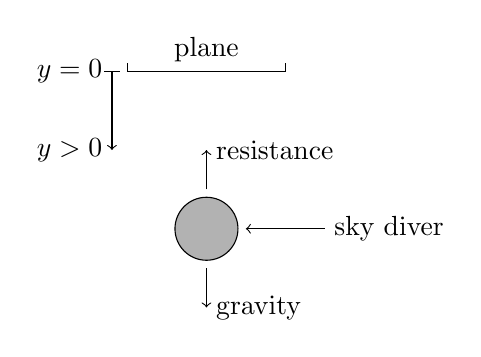
\begin{tikzpicture}
        \draw (-1,0.1) -- (-1,0) -- (1,0) -- (1,0.1);
        \draw (0,0) node[anchor=south]{plane};
        \draw[fill=black!30] (0,-2) circle(0.4cm);
        \draw[<-] (0.5,-2) -- (1.5,-2) node[anchor=west]{sky diver};
        \draw[->] (0,-1.5) -- (0,-1) node[anchor=west]{resistance};
        \draw[->] (0,-2.5) -- (0,-3) node[anchor=west]{gravity};
        \draw (-1.3,0) -- (-1.1,0);
        \draw[->] (-1.2,0) node[anchor=east]{$y=0$} -- (-1.2,-1) node[anchor=east]{$y>0$};
    \end{tikzpicture}
\end{center}

\begin{enumerate}
    \item[(a)] It can be shown experimentally that the air resistance is proportional to the
    square of the velocity.  What differential equation models the \underline{velocity} of
    the falling sky diver? \\(Hints: (1) Recall that if $y(t)$ is the position of the
    falling sky diver then $v(t) = y'(t)$ is the velocity and $a(t) = v'(t) = y''(t)$
    is the acceleration.  \\(2) be sure to get the signs correct!)
    \[ m \cdot \underline{\hspace{0.5in}} = \underline{\hspace{1in}} +
        \underline{\hspace{1in}} \]
        \solution{$mv' = mg - bv^2$}

    \item[(b)] What is the equilibrium solution to the differential equation that you
    proposed in part (a). Discuss the meaning of this equilibrium in the context of the
    problem. Is it stable or unstable? 
    \solution{
        \[ 0 = mg - bv^2 \quad \implies \quad v_{eq} = \sqrt{mg/b} \]
        This is the terminal velocity of the falling sky diver.  This is a stable
        equilibrium.
    }


\item[(c)] Sketch a plot of the velocity and the position functions vs time.  (You do
    not need to solve the differential equation.)
    \begin{center}
        \begin{tikzpicture}[scale=1]
            \begin{axis}[axis lines=center, grid, xmin=0, xmax=2, ymin=0, ymax=4,
                title={Velocity vs. Time}, xlabel={$t$}, ylabel={$v(t)$}, xtick=\empty,
            ytick=\empty]
                \addplot[smooth, black, domain=0:2] {0*x};
%                 \ipa{\addplot[smooth, very thick, red, domain=0:2] {1.96- 1.96*exp(-5*x)};}
            \end{axis}
        \end{tikzpicture}\hspace{0.2in}
        \begin{tikzpicture}[scale=1]
            \begin{axis}[axis lines=center, grid, xmin=0, xmax=2, ymin=0, ymax=4,
                title={Position vs. Time}, xlabel={$t$}, ylabel={$y(t)$}, xtick=\empty,
            ytick=\empty]
                \addplot[smooth, black, domain=0:2] {0*x};
            \end{axis}
        \end{tikzpicture}
    \end{center}


\end{enumerate}
\end{problem}




\begin{problem}[The Combustion Problem]
    Let $T$ be the temperature of a combustible material (e.g. oily rags, dry hay, etc.).
    The conservation of energy equation states that 
    \[ \rho c_p \frac{dT}{dt} = A_1 e^{-B/(T-T_0)} - h\left( T - T_a \right) \]
    where 
    \begin{itemize}
        \item $T$ is temperature in Kelvin,
        \item $T_0$ is a reference temperature above which the fuel starts oxidizing,
        \item $T_a$ is the ambient temperature of the surrounding air,
        \item $\rho$ is the density of the fuel,
        \item $c_p$ is the specific heat of the fuel source, 
        \item $h$ is a measure of the power per volume per degree Kelvin,
        \item $A_1$ is a measure of the power per unit volume, and
        \item $B$ is a rate constant measured in degrees Kelvin.
    \end{itemize}
    If we divide both sides of the differential equation by $\rho c_p$ we arrive at the
    first order non-homogeneous differential equation
    \[ \frac{dT}{dt} = A e^{-B/(T-T_0)} - C \left( T - T_a \right). \]  
    Assume that $A, B,$ and $C$ are all positive coefficients.
    \\{\bf Your Tasks:}
    \begin{enumerate}
        \item[(a)] Why must $T > T_0$ in order for the equation to make sense physically?
        \item[(b)] Let's suppose that $T_a = 300^\circ K$ and that $T_0$ is also at the
            ambient temperature.  Let $A = 20$, $B = 600$, and $C = 0.01$.  Analyze the
            differential equation graphically plotting the phase portrait, identifying
            equilibrium points, and discussing stability of each point.
        \item[(c)] Discuss the physical interpretation of each equilibrium point.
        \item[(d)] Suppose we don't know what $A$, $B$, and $C$a re, but we do know from
            experiments that the three fixed points are $T_1 = T_a = 300^\circ K$, $T_2 =
            670^\circ K$, and $T_3 = 1200^\circ K$.  What can you say about the
            coefficients $A$, $B$, and $C$?
    \end{enumerate}
\end{problem}
\solution{
    \begin{center}
        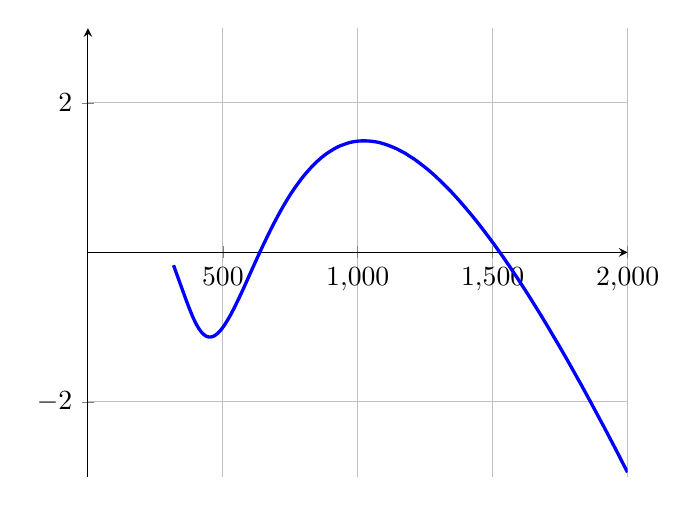
\begin{tikzpicture}
            \begin{axis}[axis lines=center, grid, xmin=0, xmax=2000, ymin=-3, ymax=3,
                domain=300:2000]
                \addplot[smooth, very thick, blue, samples=100] {20*exp(-600/(x-300)) - 0.01*(x-300)};
            \end{axis}
        \end{tikzpicture}
    \end{center}
    The fixed points are $T_1 = 300^\circ K$, $T_2 \approx 636.8^\circ K$, and $T_3
    \approx 1526^\circ K$.  $T_1$ is stable from the right, $T_2$ is unstable (above which
    a combustion occurs), and $T_3$ is stable (stable combustion).
}



